\subsubsection{Harvester-Tarpit}
Um Harvester in die Falle zu locken besitzt VEVETA zwei Methoden:
\begin{enumerate}
	\item Generieren einer E-Mail-Adresse anhand der IP-Adresse
	\item Generieren verschiedener E-Mail-Adressen
\end{enumerate}
\paragraph{Generieren einer E-Mail-Adresse anhand der IP-Adresse}\mbox{}\\
Dem Aufrufer wird auf der Landingpage\footnote{Als Landingpage wird in der Regel jene Webseite bezeichnet, welche beim Aufruf einer URL als erstes angezeigt wird} neben einem Kontaktformular eine E-Mail-Adresse angezeigt, welche folgende Form aufweist: \emph{[IP-ADRESSE]-[DATUM]-[UHRZEIT]@maturaprojekt.ddns.net}.\\
Damit Harvester diese E-Mail-Adresse auch schnell finden, wurde sie mit dem Schlüsselwort \emph{mailto:} gekennzeichnet, das in HTML als Kennzeichen für eine E-Mail-Adresse verwendet wird. Der Code zum generieren dieser E-Mail-Adresse ist in der Datei \emph{index.php} inkludiert:\\
\lstinputlisting[language=PHP, firstline=378, lastline=389]{sourcefiles/index.php}
Ein Aufruf der Datei index.php würde beispielsweise folgende E-Mail-Adresse generieren:
\emph{82.52.47.189-02.04.2018-16.20.58@maturaprojekt.ddns.net}, welche aus den Augen eines Harvesters folgende HTML-Struktur aufweist:\\
\lstinputlisting[language=HTML]{sourcefiles/generated-mail.html}
\paragraph{Generieren verschiedener E-Mail-Adressen}\mbox{}\\
Des Weiteren generiert das Skript \emph{reply.php}, wie unter Punkt \ref{subsub:hyperlink-tarpit} beschrieben, auch E-Mail-Adressen. Wie unter demselben Punkt erwähnt, besteht die ein-prozentige Chance, dass ein Hyperlink generiert wird. Wenn dieser Fall eintritt, besteht des Weiteren eine zehn-prozentige Chance, dass anstelle eines Hyperlinks eine E-Mail-Adresse generiert wird. Somit wird mit einer Wahrscheinlichkeit von 0,1\% eine E-Mail-Adresse vom Skript generiert. Dies entspricht in etwa fünf bis zehn E-Mail-Adressen pro generierter Webseite. Um diese E-Mail-Adressen so realistisch als möglich aussehen zu lassen, wurden online auf der Webseite \url{http://www.freedatagenerator.com/csv-data-generator} E-Mail-Adressen generiert, von denen eine mit einer Wahrscheinlichkeit 50\% ausgewählt wird; ansonsten wird eine E-Mail-Adresse bestehend aus zufälligen Zeichen generiert. Bei beiden Varianten wird vorne an der E-Mail-Adresse die Zeit zum Zeitpunkt des Generierens in Form eines Unix-Timestamps\footnote{Der Unix-Timestamp ist eine einfache, aber dennoch exakte Art Zeit zu messen. Der Unix-Timestamp besteht aus einer Zahl, welche die Anzahl an Sekunden, die seit dem 1. Januar 1970 vergangen sind, angibt.} angefügt.\\
Die Verteilung der Ausgabe des Skriptes reply.php ist in der Abbildung \ref{fig:wahrbaum} aufgeführt.\\
Alle E-Mail-Adressen verweisen auf die Domain \emph{@maturaprojekt.ddns.net} und landen somit auf einem Mail-Server, welcher neben dem Apache-Webserver auf dem Raspberry Pi läuft.\\
Diese Form der Tarpit dient in erster Linie dazu, Harvester zu entlarven und ihre Mailinglisten mit unsinnigen E-Mail-Adressen zu verstopfen. Durch das Anhängen des Timestamps kann man im Nachhinein herausfinden, welche IP-Adresse und welcher User-Agent zu einem Harvester gehörte, da man diese in den Logfiles beim Eintrag, dessen Zeit zum Timestamp korrespondiert, ablesen kann. Da der Timestamp jedoch erst nachträglich eingefügt wurde, können nicht mehr alle E-Mail-Adressen einem Harvester zugeordnet werden.
\begin{figure}[H]
	\centering
	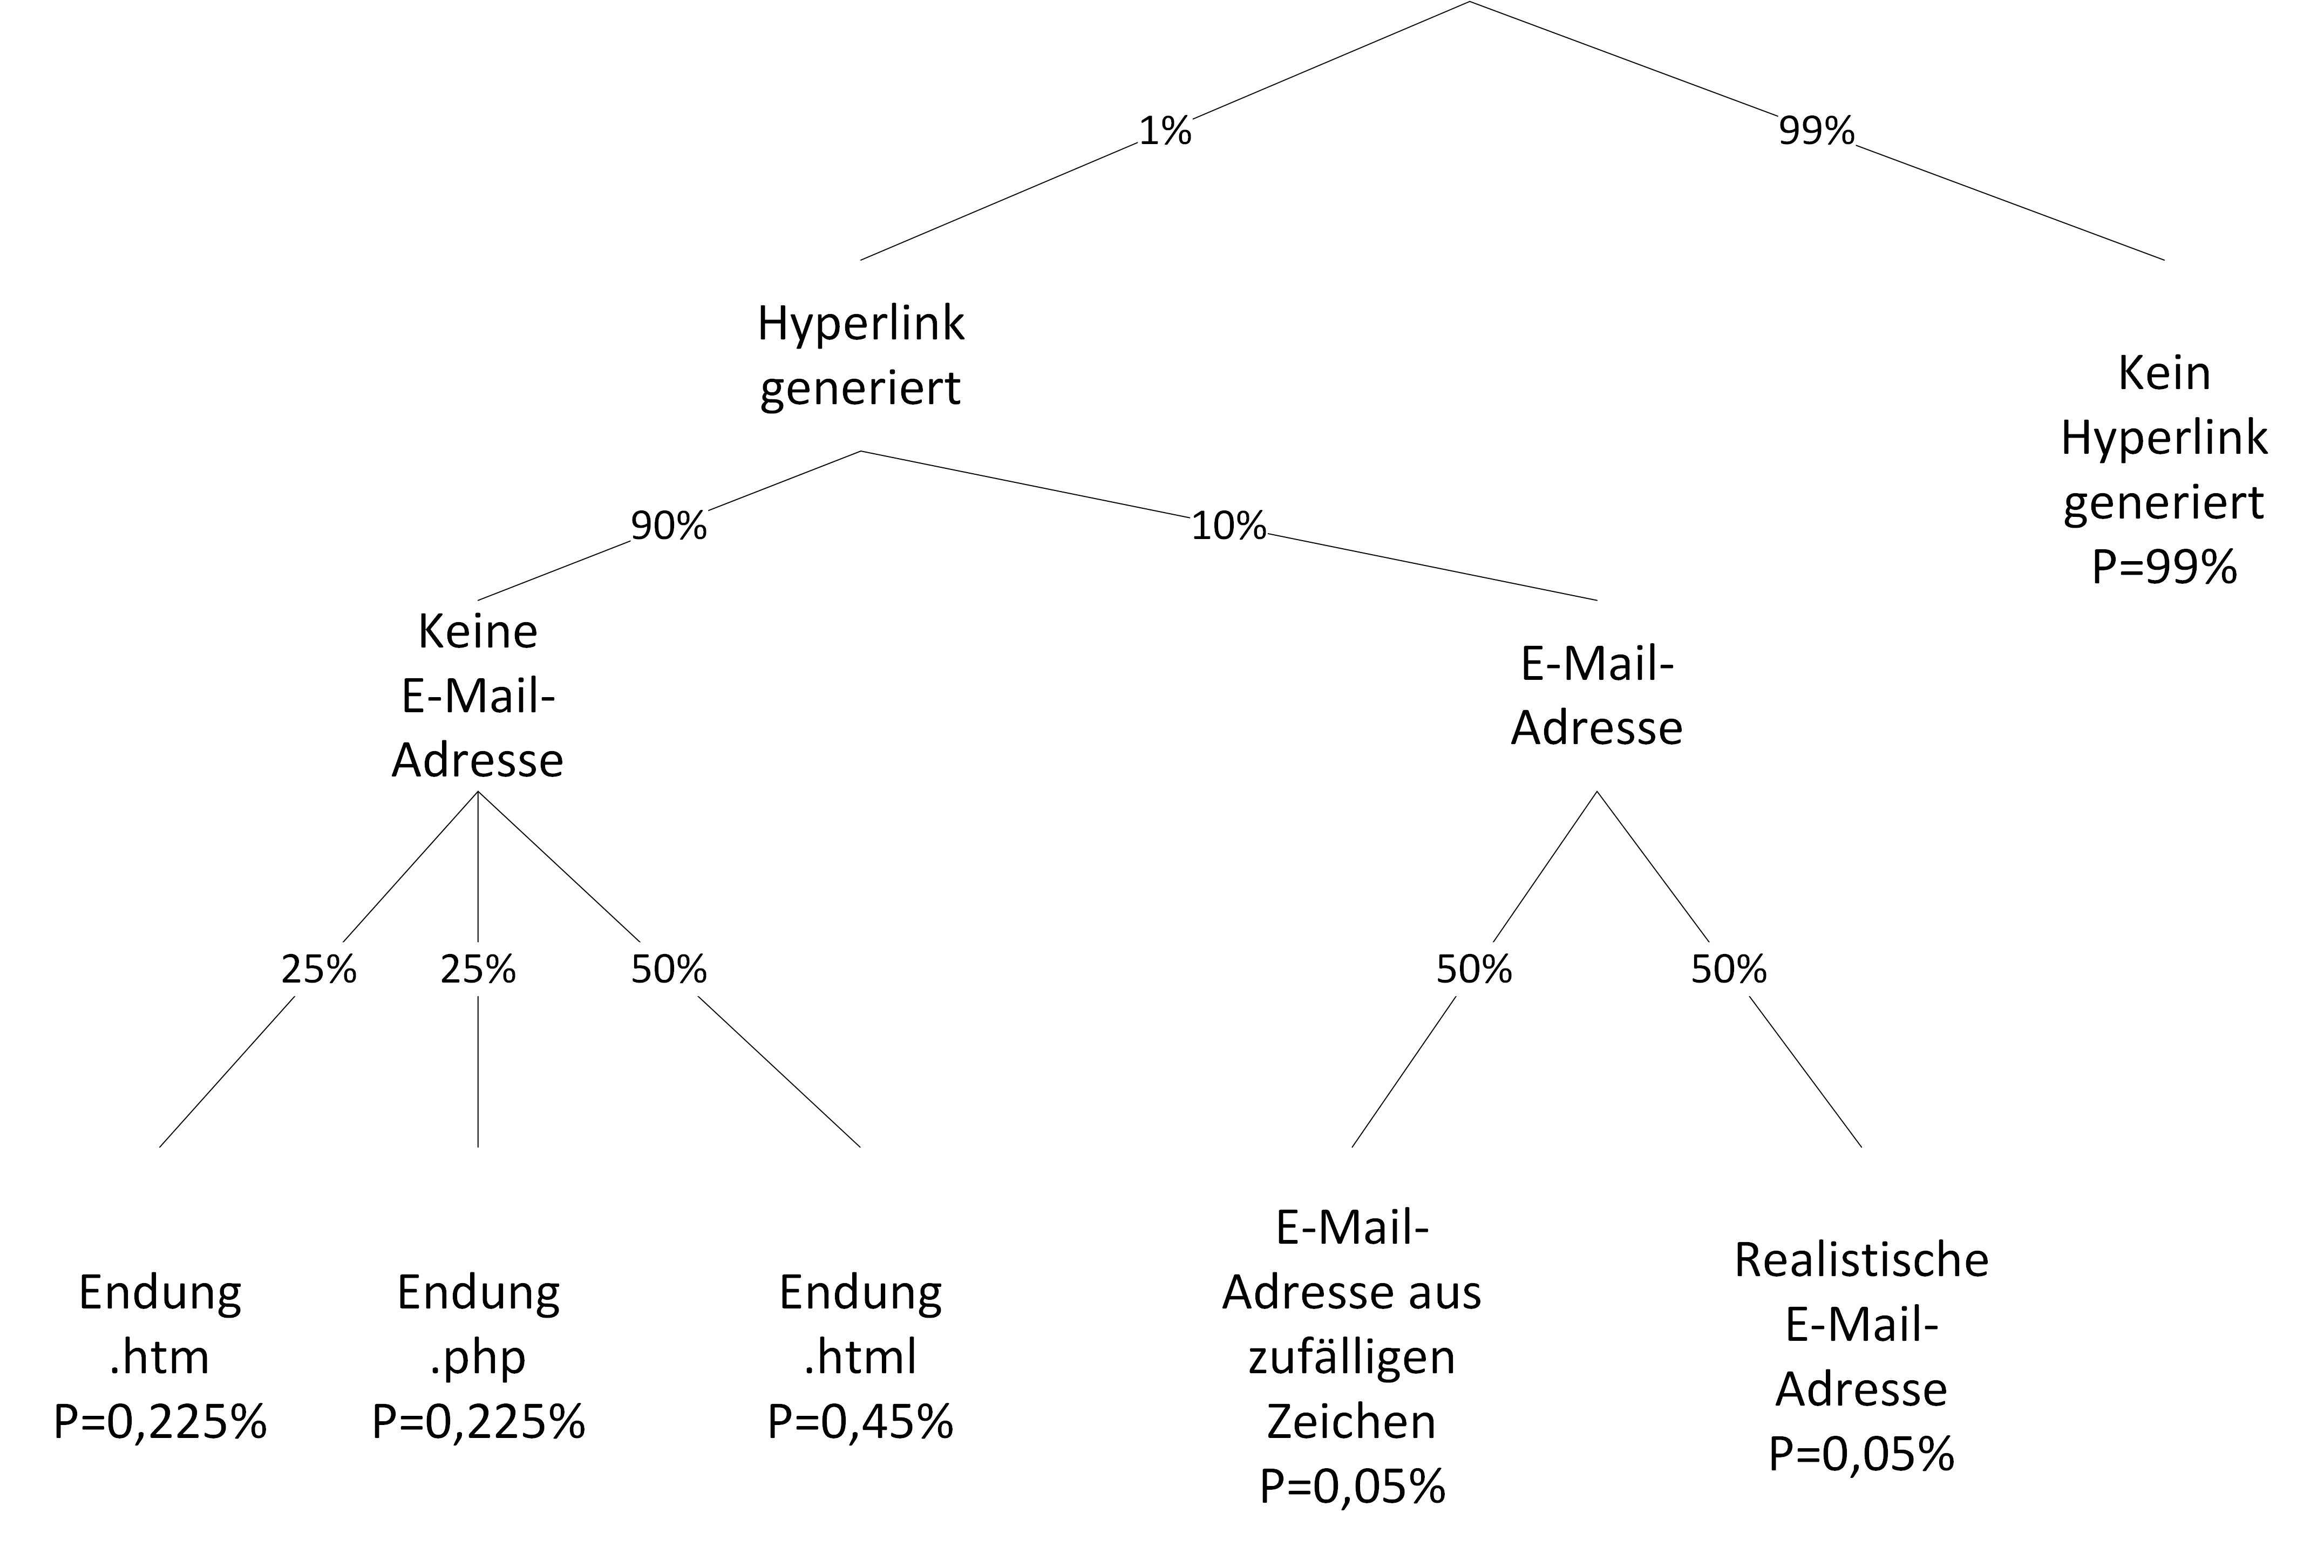
\includegraphics[width=8.45cm]{img/Wahrscheinlichkeitsbaum.png}
	\caption{Wahrscheinlichkeitsbaum der Ausgabe des Skriptes \emph{reply.php}. Die Wahrscheinlichkeit ist am jeweils letzten Blatt eines Astes angeführt. \emph{P} entspricht hier der Wahrscheinlichkeit}
	\label{fig:wahrbaum}
\end{figure}
%% The sloped option gives rotated edge labels. Personally
% I find sloped labels a bit difficult to read. Remove the sloped options
% to get horizontal labels. 
\begin{tikzpicture}[grow=down]
\node[bag] {}
    child {
        node[bag] {Hyperlink generiert}        
            child {
                node[bag] {E-Mail-Adresse}
                child {
                	node[end, label=below:
                	{E-Mail-Adresse aus zufällig generierten Zeichen}] {}
                	edge from parent
                	node[below]  {50\%}
                }
                child {
                	node[end, label=below:
                	{realistische E-Mail-Adresse}] {}
                	edge from parent
                	node[below]  {50\%}
                }
                edge from parent
                node[below]  {10\%}
            }
            child {
            	node[bag] {keine E-Mail-Adresse}
            	child {
            		node[end, label=below:
            		{Endung .htm}] {}
            		edge from parent
            		node[below]  {25\%}
            	}
	            child {
	            	node[end, label=below:
	            	{Endung .php}] {}
	            	edge from parent
	            	node[below]  {25\%}
	            }
            	child {
            		node[end, label=below:
            		{Endung .html}] {}
            		edge from parent
            		node[below]  {50\%}
            	}
            	edge from parent
            	node[below]  {90\%}
            }
            edge from parent 
            node[below]  {1\%}
    }
    child {
        node[end, label=below:
        {kein Hyperlink generiert}] {}
        edge from parent
        node[below]  {99\%}
    };
\end{tikzpicture}
\label{subsub:harverster-tarpit}
